\documentclass[%
	paper=A4,	% stellt auf A4-Papier
	pagesize,	% gibt Papiergröße weiter
	DIV=calc,	% errechnet Satzspiegel
	smallheadings,	% kleinere Überschriften
	ngerman		% neue Rechtschreibung
]{scrartcl}
\usepackage{BenMathTemplate}
\usepackage{BenTextTemplate}

\title{{\bf Wissenschaftliches Rechnen III / CP III}\\Übungsblatt 4}
\author{Tizia Kaplan (545978)\\Benjamin Dummer (532716)\\ Gruppe 10}
\date{25.05.2016}

\begin{document}
\maketitle
Online-Version: \href{https://www.github.com/BeDummer/CP3_UE4}{\url{https://www.github.com/BeDummer/CP3_UE4}}

\section*{Aufgabe 4.i}
Hier sollten die Laufzeiten f"ur $n=2^24$ Elemente f"ur unterschiedliche Blockgr"o\ss en mithilfe von \texttt{nvprof ./a.out} gemessen werden. Vergleichend wurden die elapsed Zeiten f"ur die Implementierung \texttt{reduceInterleaved} und \texttt{reducedUnrolling} aufgenommen. Gefunden wurde ein Minimum bei Blocksize $=128$ (siehe Abb. 1) 

\section*{Aufgabe 4.ii}
Nun konnten auch Global Load Throughput, Global Load Efficiency und Achieved Occupancy gemessen werden. Hier wurden mittels \texttt{nvprof --metrics gld_efficiency,gld_throughput,achieved_occupancy ./a.out} die Durchschnittswerte ermittelt.
ABBILDUNGEN

\section*{Aufgabe 4.iii}
Man erkennt eine Laufzeitverbesserung f"ur Blockgr"o\ss en $\leq 128$ und erreicht dort ein Minimum. Die Verbesserung wird auch deutlich durch steigende Werte der in ii) gemessenen Parameter. Ab Blocksize $128$ jedoch, "andern sich die Load Efficiency und die Achieved Occupancy nur unwesentlich - die Bandbreite sinkt jedoch wieder ab. Dementsprechend gibt es ein Minimum der Laufzeit bei Blockgr"o\ss e $128$.

In Abb.1 l"asst sich au\ss erdem noch eine starke Differenz der Laufzeiten zwischen Interleaved und Unrolling erkennen. Unter einer Blockgr"o\ss e von $128$ ist die Load Efficiency ausschlaggebend f"ur die Laufzeitunterschiede. Danach nimmt die Bandbreite den entscheidenden Einfluss auf die Differenz.

\section*{Aufgabe 4.iv}
Hier wurde q als Potenz von $2$ implementiert. Das Optimum der Laufzeit wurde f"ur fast alle Blockgr"o\ss en (analog zu i) ) bei $q=2^11=2048$ gefunden. Nur bei Blockgr"o\ss e $32$ wurde ein $q=4096$ erhalten. Auffallend war, dass q auch hier einen Einfluss auf die absolute Laufzeit der unterschiedlichen Blockgr"o\ss en hatte: im Test wurde die schnellste Laufzeit von $t_{unrollOpt}=1.42 ms$ f"ur eine Blocksize von $1024$ gefunden.

\section*{Aufgabe 4.v}
Ausgehend von unserer Analyse in iv) haben wir nun also unsere optimierte Reduktion f"uer den Datentyp \texttt{double} mit der besten Blockgr"o\ss e $1024$ und dem optimalen $q=2048$ erweitert.


\begin{figure}
  \centering
  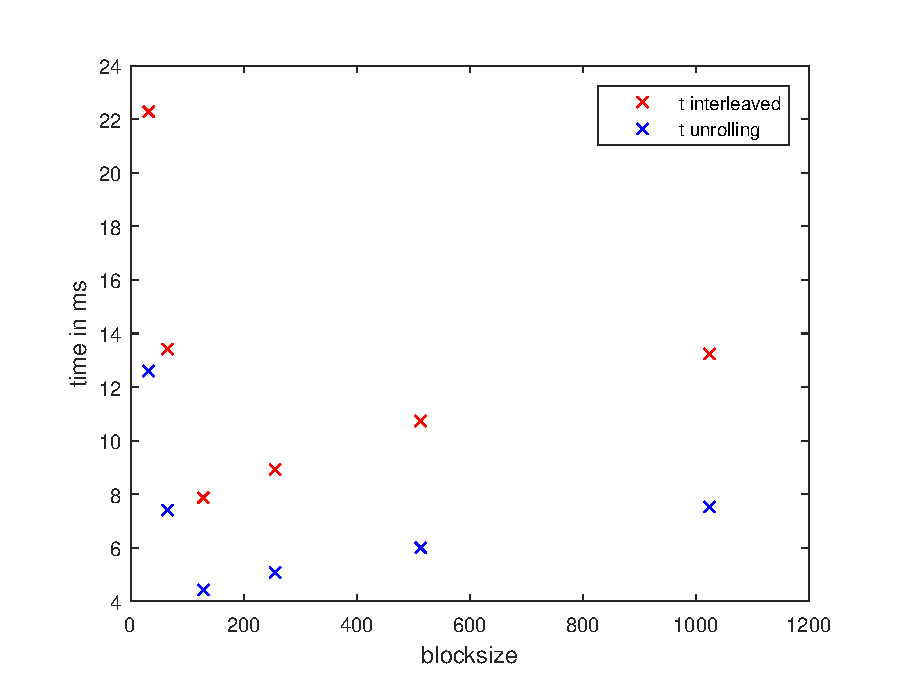
\includegraphics[width=.8\textwidth]{blocksize_vs_time_interl_unroll.eps}
  \caption{Blocksize vs. Simulationszeit f"ur die unterschiedlichen Realisierungen der parallelen Reduktion (interleaved \& unroll)}
\end{figure}

\begin{figure}
  \centering
  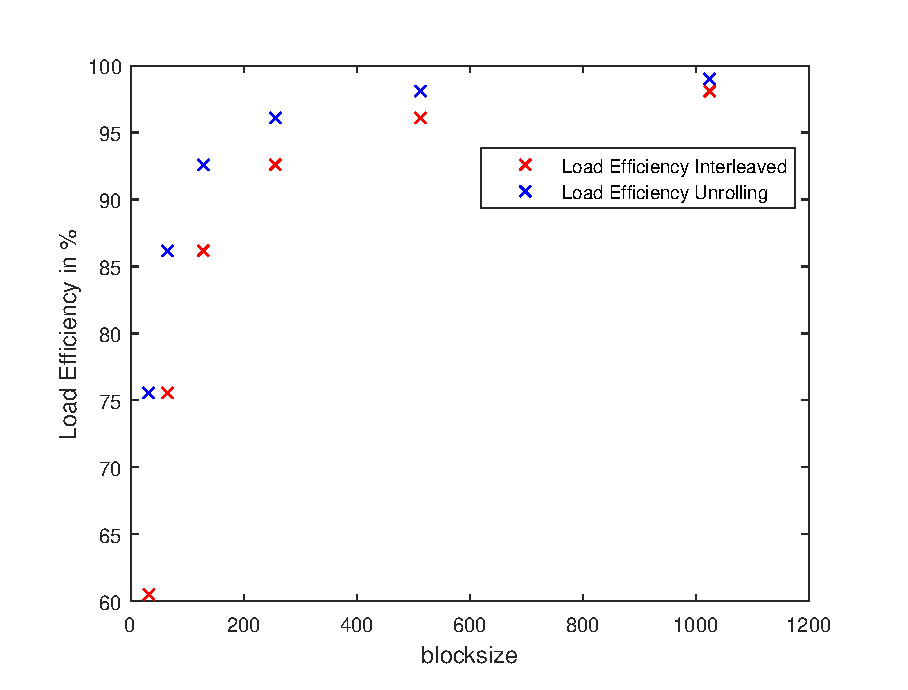
\includegraphics[width=.8\textwidth]{blocksize_vs_load_efficiency.eps}
  \caption{Blocksize vs. Global Load Efficiency f"ur die unterschiedlichen Realisierungen der parallelen Reduktion (interleaved \& unroll)}
\end{figure}

\begin{figure}
  \centering
  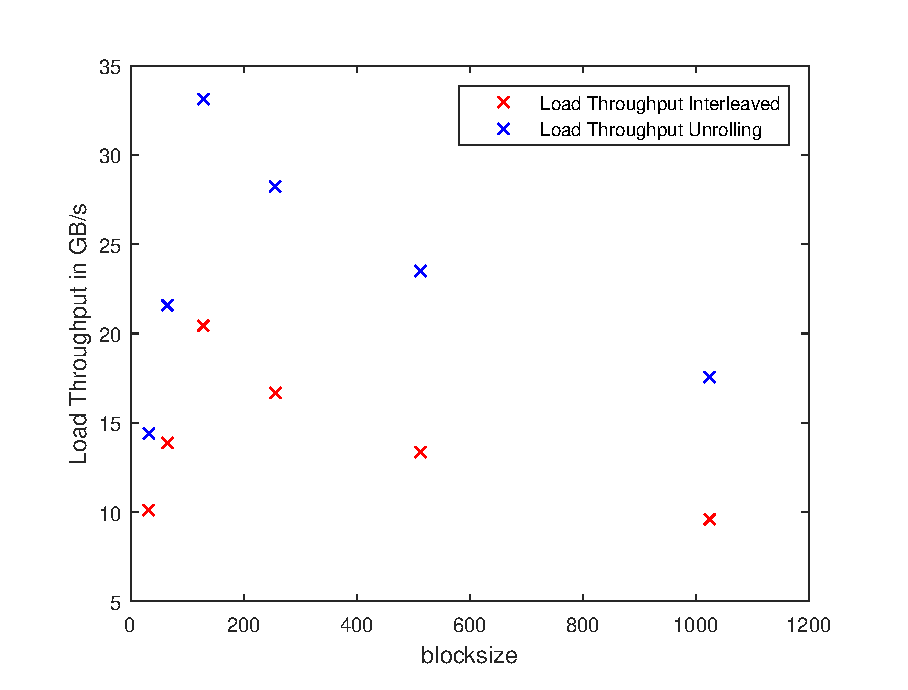
\includegraphics[width=.8\textwidth]{blocksize_vs_load_throughput.eps}
  \caption{Blocksize vs. Global Load Throughput (Bandbreite) f"ur die unterschiedlichen Realisierungen der parallelen Reduktion (interleaved \& unroll)}
\end{figure}

\begin{figure}
  \centering
  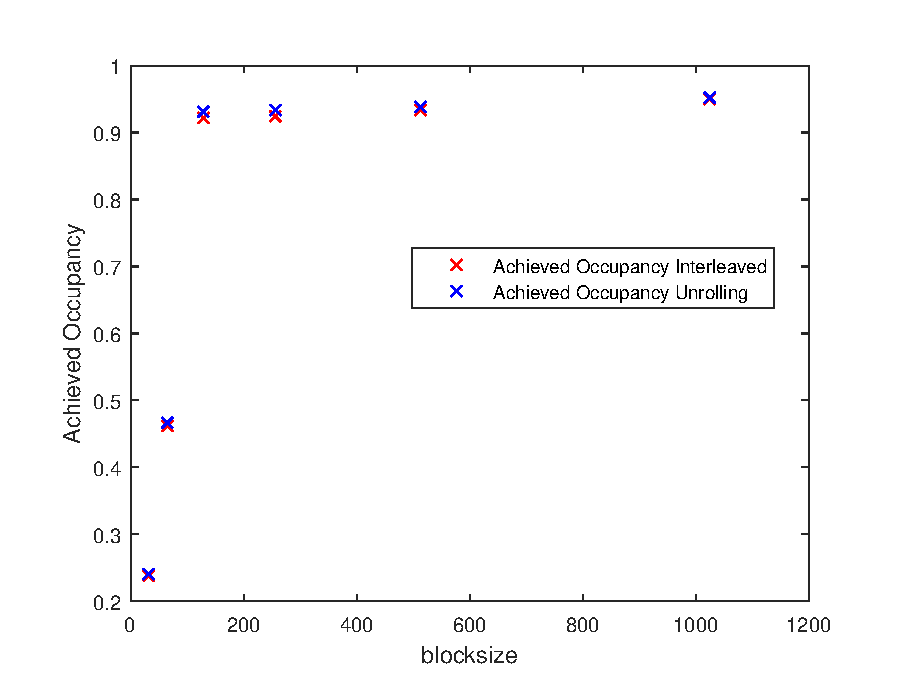
\includegraphics[width=.8\textwidth]{blocksize_vs_achieved_occ.eps}
  \caption{Blocksize vs. Achieved Occupancy f"ur die unterschiedlichen Realisierungen der parallelen Reduktion (interleaved \& unroll)}
\end{figure}

\section*{Anhänge}
\begin{itemize}
	\item Datei: \url{reduction_w_q.cu} (Hauptprogramm)
\end{itemize}
\end{document}
